\subsection{Hoofdprotocol}
Hier wordt het protocol besproken tussen de gebruikerapplicatie en de twee servers als de gebruiker aanbevelingen vraagt. Alvorens het aanvragen van aanbevelingen slaat een gebruiker zijn beoordelingen en voorkeuren op en stuurt ze dan samen in zijn profiel naar de recommenderserver (\ref{voor_aanvraag}). Eens gebruiker 1 aanbevelingen vraagt is de eerste stap de gelijkenisfactor berekenen tussen gebruiker 1 en de andere gebruikers Ux. Dit gebeurt door de aanbevelingsserver in paragraaf \ref{similarities}.  Daarna gaat de server met het thresholdprotocol (\ref{threshold}) na of deze ge\"encrypteerde waarden boven een drempelwaarde liggen. Nu bezit de recommender een ge\"encrypteerde bit per gebruiker die aangeeft of dit wel (1) of niet (0) het geval is. Hierop starten de recommender en de privacy provider een nieuw protocol waarbij de controleserver een deel van de gebruikers selecteert die kunnen meedoen aan het protocol (\ref{selection}). De resultaatbits hiervan geven aan of de ratings van respectievelijke gebruiker zullen worden meegeteld in het berekenen van de aanbevelingen. Het multiplicationprotocol (\ref{multiplication}) vermenigvuldigt deze gebruikerbits met zijn overeenkomstige ratings. Daarna wordt de som van de ratings per item genomen over alle gebruikers heen in paragraaf \ref{sumoverallusers} en wordt het resultaat privacyvriendelijk naar de gebruiker gebracht (\ref{result}). Dit is de code van het protocol op de recommenderserver : 

\begin{verbatim}
@POST
@Path("recommendations")
@Produces({"application/json"})
@Consumes({"application/json"})
public ResultDAO getRecommendations(RecommendationDAO rd)... {    
	...
    //berekenen van gelijkeniswaarden
    SimDAO sDao = getSimilarities((User) q.getSingleResult(),
    pubKeyPaillierControlServer);
    LinkedHashMap<Integer,EncryptedInteger> similarities = sDao.getSimilarities();
    //vergelijken gelijkeniswaarden met drempelwaarde
    EncryptedInteger threshold =new EncryptedInteger (new BigInteger(thres),
    		pubKeyPaillierControlServer);
    similarities = compare(similarities,threshold,
        pubKeyPaillierControlServer,pubKeyDGKControlServer.getL());
	//selecteren gebruikers door de controleserver    
    similarities =
    		HTTPClient.exchangeDeltas(simularities,pubKeyPaillierControlServer);          
    sDao.setSimilarities(similarities);
    //resultaatbits vermenigvuldigen met ratings overeenkomstige users  
    //plus sommeren over alle items heen
    sDao = multiplySimilaritiesWithRatings(sDao,pubKeyPaillierControlServer);
    //uitwisselen resultaten met behulp van randomwaarden
    rd = exchangeResults(rd,sDao,pubKeyPaillierControlServer);
    return getItems(rd,sDao);
    }
\end{verbatim}

Het sequentiediagram \ref{Figuur::hoofdprotocoldiagram} geeft de communicatie weer tussen de clientapplicaties en de twee servers als een gebruiker aanbevelingen vraagt. De paragrafen waar de onderdelen ervan besproken worden staan links aangegeven. Functies, protocollen en taken staan in het zwart aangegeven, attributen in het blauw. De berekeningen op de aanbevelingsserver gebeuren in het gesloten Pailliersysteem getekend met publieke sleutel S2 zodat de server geen persoonlijke data kan lezen.

\begin{center}
\centering
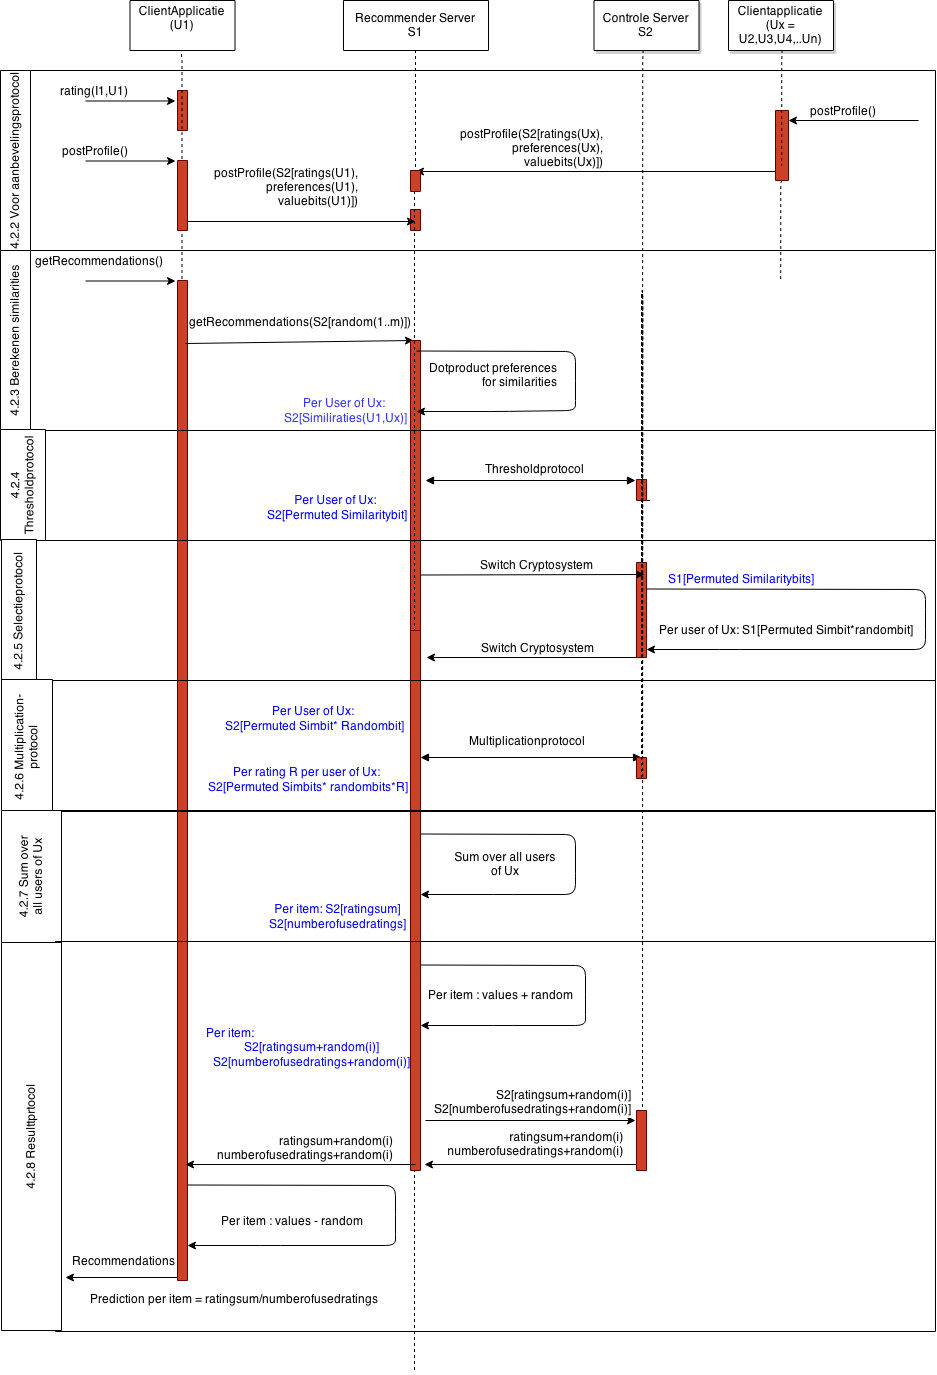
\includegraphics[width=1.0\textwidth,keepaspectratio]{fig/hoofdprotocol_privacy}   %
\label{Figuur::hoofdprotocoldiagram}%
\end{center}



